\documentclass[aspectratio=169]{beamer}
\usetheme{Madrid}
\usecolortheme{default}

\usepackage{amsmath}
\usepackage{amssymb}
\usepackage{tikz}
\usetikzlibrary{shapes.geometric, arrows.meta, positioning, fit, backgrounds}
\usepackage{xcolor}
\usepackage{booktabs}
\usepackage{graphicx}
\usepackage{hyperref}

\definecolor{success}{RGB}{46, 125, 50}
\definecolor{warning}{RGB}{255, 152, 0}
\definecolor{error}{RGB}{211, 47, 47}
\definecolor{info}{RGB}{2, 136, 209}
\definecolor{s1color}{RGB}{33, 150, 243}
\definecolor{s2color}{RGB}{156, 39, 176}
\definecolor{s3color}{RGB}{76, 175, 80}
\definecolor{s4color}{RGB}{255, 152, 0}
\definecolor{s5color}{RGB}{233, 30, 99}

\newcommand{\cmark}{\textcolor{success}{\checkmark}}
\newcommand{\xmark}{\textcolor{error}{$\times$}}

\title[PostProcessing\_evaluator]{PostProcessing\_evaluator}
\subtitle{An isolated workspace to build publication-ready postprocessing\\\small{Field inventory, SWC sampling, front-aware analysis --- without touching the official pipeline}}
\author{Nicole Flores}
\institute{KAUST}
\date{\today}

\begin{document}

\frame{\titlepage}

\begin{frame}{Outline}
\tableofcontents
\end{frame}

%=============================================================================
\section{Why a PostProcessing evaluator}

\begin{frame}{Why this evaluator exists}
\begin{block}{Goal}
Develop and validate postprocessing tools that extract time-dependent values
along simulated neuronal geometries, and identify quantities + figures
suitable for publication.
\end{block}

\begin{alertblock}{Problem with the old organization}
The original outputs landed under \texttt{/scratch/flore0a/AnalysisResults/}
without timestamps, without a manifest, and without a clean separation
between raw and enriched data. Scripts were duplicated in two locations
(\texttt{Postanalysis\_swc/} and \texttt{Value\_Extraction/}, byte-identical).
\end{alertblock}

\begin{block}{Approach}
Stand up an evaluator workspace that \textbf{leaves the official pipeline
untouched} and produces \textbf{timestamped, manifested} outputs to scratch.
The official pipeline remains the ground-truth reference until the evaluator
is validated.
\end{block}
\end{frame}

%=============================================================================
\section{What is protected}

\begin{frame}{Hard boundaries}
\begin{block}{Never modified}
\begin{itemize}
  \item \texttt{/project/.../plugins/Growth\_Plugin/python\_utils/PostProcessing} \\
        --- the official Python postprocessing pipeline.
  \item \texttt{/project/.../apps/Neuronal\_Process/PostProcessing} \\
        --- the older app-side mirror.
  \item \texttt{/project/.../apps/Neuronal\_Process/Scripts\_lua/Model\_only\_final\_steps.lua} \\
        --- and any production Lua.
  \item \texttt{/scratch/flore0a/AnalysisResults} \\
        --- historical postprocessing outputs (read-only reference).
\end{itemize}
\end{block}

\begin{block}{Allowed}
\begin{itemize}
  \item Read everything above.
  \item Write only inside \texttt{/project/.../PostProcessing\_evaluator/} \\
        and \texttt{/scratch/flore0a/PostProcessing\_evaluator/}.
\end{itemize}
\end{block}
\end{frame}

%=============================================================================
\section{Evaluator structure}

\begin{frame}[fragile]{Layout (project side)}
\small
\begin{verbatim}
PostProcessing_evaluator/
  README.md
  copied_reference/                    (frozen, chmod 0444)
    README_PROVENANCE.md
    old_analysisresults_scripts/       (the 4 scripts that
                                        produced AnalysisResults)
  scripts/
    inspect_simulation_fields.py       (NEW; autodetect fields)
    reproduction/
      run_chain.py                     (NEW; orchestrator)
  sh_files/                            (login-node runners)
  slurm/                               (Shaheen jobs; srun+pvpython)
  presentation/
  configs/, reports/, tests/, logs/
\end{verbatim}
\end{frame}

\begin{frame}[fragile]{Layout (scratch side)}
\small
\begin{verbatim}
/scratch/flore0a/PostProcessing_evaluator/
  inputs/    outputs/    figures/    tables/
  reports/                  (timestamped MD + CSV reports)
  runs/<TS>/                (one inspection run per timestamp)
  reproduction_runs/<TS>/   (one full reproduction per timestamp)
  logs/                     (SLURM and login-node logs)
  temporary/
\end{verbatim}

Every output directory carries a \texttt{YYYYMMDD\_HHMMSS} stamp.
The historical \texttt{AnalysisResults/} is never written to.
\end{frame}

%=============================================================================
\section{First-pass field inventory}

\begin{frame}{Stage 1: \texttt{inspect\_simulation\_fields.py}}
\begin{block}{What it does}
Read-only inspection of one simulation directory.
\begin{itemize}
  \item Autodetects \texttt{Simulation.vtkhdf}, \texttt{merged/Output\_t*.vtu},
        \texttt{*.pvtu}.
  \item Enumerates timesteps and time values.
  \item For every point-data, cell-data, and field-data array: reports
        \(\min, \max, \text{mean}, \text{std}, n_{\text{tuples}}\), and
        counts of NaN / Inf.
  \item Vector arrays are reported per-component plus magnitude.
\end{itemize}
\end{block}

\begin{block}{Outputs}
\texttt{/scratch/.../PostProcessing\_evaluator/runs/<TS>/}
\begin{itemize}
  \item \texttt{field\_inventory.csv} --- long format.
  \item \texttt{field\_inventory.md} --- per-step compact tables.
  \item \texttt{run\_metadata.json} --- command, executable, VTK version, hostname.
  \item \texttt{log.txt} --- stdout/stderr mirror.
\end{itemize}
\end{block}

\textcolor{info}{Crucial: no field name is hard-coded. The script reports what is there.}
\end{frame}

%=============================================================================
\section{Recovered workflow}

\begin{frame}{Workflow stages (recovered from AnalysisResults)}
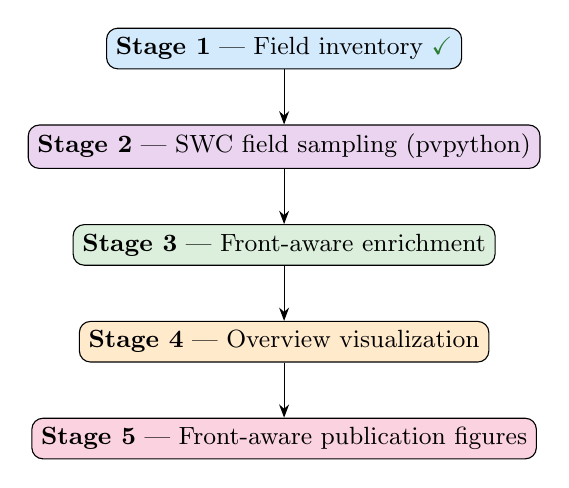
\begin{tikzpicture}[node distance=0.7cm, every node/.style={font=\small}]
\node[draw, fill=s1color!20, rounded corners, minimum width=4cm] (s1) {\textbf{Stage 1} --- Field inventory \cmark};
\node[draw, fill=s2color!20, rounded corners, minimum width=4cm, below=of s1] (s2) {\textbf{Stage 2} --- SWC field sampling (pvpython)};
\node[draw, fill=s3color!20, rounded corners, minimum width=4cm, below=of s2] (s3) {\textbf{Stage 3} --- Front-aware enrichment};
\node[draw, fill=s4color!20, rounded corners, minimum width=4cm, below=of s3] (s4) {\textbf{Stage 4} --- Overview visualization};
\node[draw, fill=s5color!20, rounded corners, minimum width=4cm, below=of s4] (s5) {\textbf{Stage 5} --- Front-aware publication figures};

\draw[-Stealth] (s1) -- (s2);
\draw[-Stealth] (s2) -- (s3);
\draw[-Stealth] (s3) -- (s4);
\draw[-Stealth] (s4) -- (s5);
\end{tikzpicture}

\vspace{0.3cm}
\small
\textbf{Stage 1} is new evaluator code. \textbf{Stages 2--5} are the 4 frozen
scripts that produced \texttt{AnalysisResults} (verified via
\texttt{IA\_session\_report\_20260503\_153249.md}).
\end{frame}

\begin{frame}{Stages 6--8 (frozen reference, deferred)}
\begin{block}{Stage 6 --- Morphometric extraction}
\texttt{compute\_morphometrics.py} (frozen). Per-frame morphometric features.
\end{block}
\begin{block}{Stage 7 --- Multivariate / statistical analysis}
\texttt{analyze\_morphometrics.py} (frozen). \(D \times V\) parameter study,
correlations, PCA, marginal effects, interaction terms.
\end{block}
\begin{block}{Stage 8 --- Mosaic / matrix visualization}
\texttt{matrix.py} (frozen). Mosaic GIF assembly across cases.
\end{block}

\textcolor{info}{Stages 6--8 need the full multi-case \texttt{Dataset\_test*}
tree, not a single case. AnalysisResults only contains D7.5\_V3.}
\end{frame}

%=============================================================================
\section{Planned analyses}

\begin{frame}{Publication-oriented analyses (planned)}
\begin{enumerate}
  \item \textbf{Front-aware kymographs} (Stage 5 \texttt{figA\_*}) ---
        tubulin / MAP2 / calcium / inhibitor along path-length over time.
  \item \textbf{Growth-cone dynamics} (\texttt{figC}) --- concentrations
        localized at the growth cone vs time; pair with elongation rate.
  \item \textbf{Elongation rate vs concentration} (\texttt{figD}) --- the
        coupling figure: \(dL/dt\) at lag-1 vs growth-cone concentration.
  \item \textbf{L\_max plateau} --- D7.5\_V3 plateaus at \(L_{\max}\approx 3.05\)
        from frame \(\sim 5\); not currently a figure but visible in
        \texttt{summary\_report.txt}.
  \item \textbf{Pixel-vs-clean skeleton agreement} --- quantitative comparison
        of the two variants (currently visual only).
  \item \textbf{Cross-case stability} --- inspect every \(D*\_V*\) in
        \texttt{Dataset\_test\{2,3,4\}}; build per-field consistency reports.
\end{enumerate}
\end{frame}

%=============================================================================
\section{Safety boundary}

\begin{frame}{Safety summary}
\begin{block}{Confirmed this session (read-only setup)}
\begin{itemize}
  \item Official PostProcessing modified: \xmark\ \textbf{NO}.
  \item AnalysisResults modified: \xmark\ \textbf{NO}.
  \item Production Lua modified: \xmark\ \textbf{NO}.
  \item Existing results overwritten: \xmark\ \textbf{NO}.
  \item Frozen reference (\texttt{copied\_reference/}) \texttt{chmod 0444}.
\end{itemize}
\end{block}

\begin{block}{Standing operational rules followed}
\begin{itemize}
  \item All SLURM scripts: \texttt{--mail-user=elsanicole.florespretell@kaust.edu.sa},
        \texttt{--mail-type=ALL}.
  \item All compute-node writes to \texttt{/scratch/} only.
  \item All pvpython invocations under \texttt{srun --ntasks=1}.
  \item All outputs timestamped \texttt{YYYYMMDD\_HHMMSS}.
\end{itemize}
\end{block}
\end{frame}

\begin{frame}{Next steps (await user authorization)}
\begin{enumerate}
  \item Submit Stage 1 inspection on D7.5\_V3 (\texttt{sbatch run\_inspect\_simulation\_fields.slurm}).
  \item Submit reproduction (\texttt{VARIANT=clean} first; then \texttt{pixel}).
  \item Generate \texttt{reproduction\_comparison\_<TS>.md} comparing reproduced
        outputs vs \texttt{/scratch/flore0a/AnalysisResults}.
  \item Extend to additional \(D*\_V*\) cases.
\end{enumerate}
\end{frame}

\end{document}
